\section*{Figure captions}

\begin{figure}[h!]
  \centering
	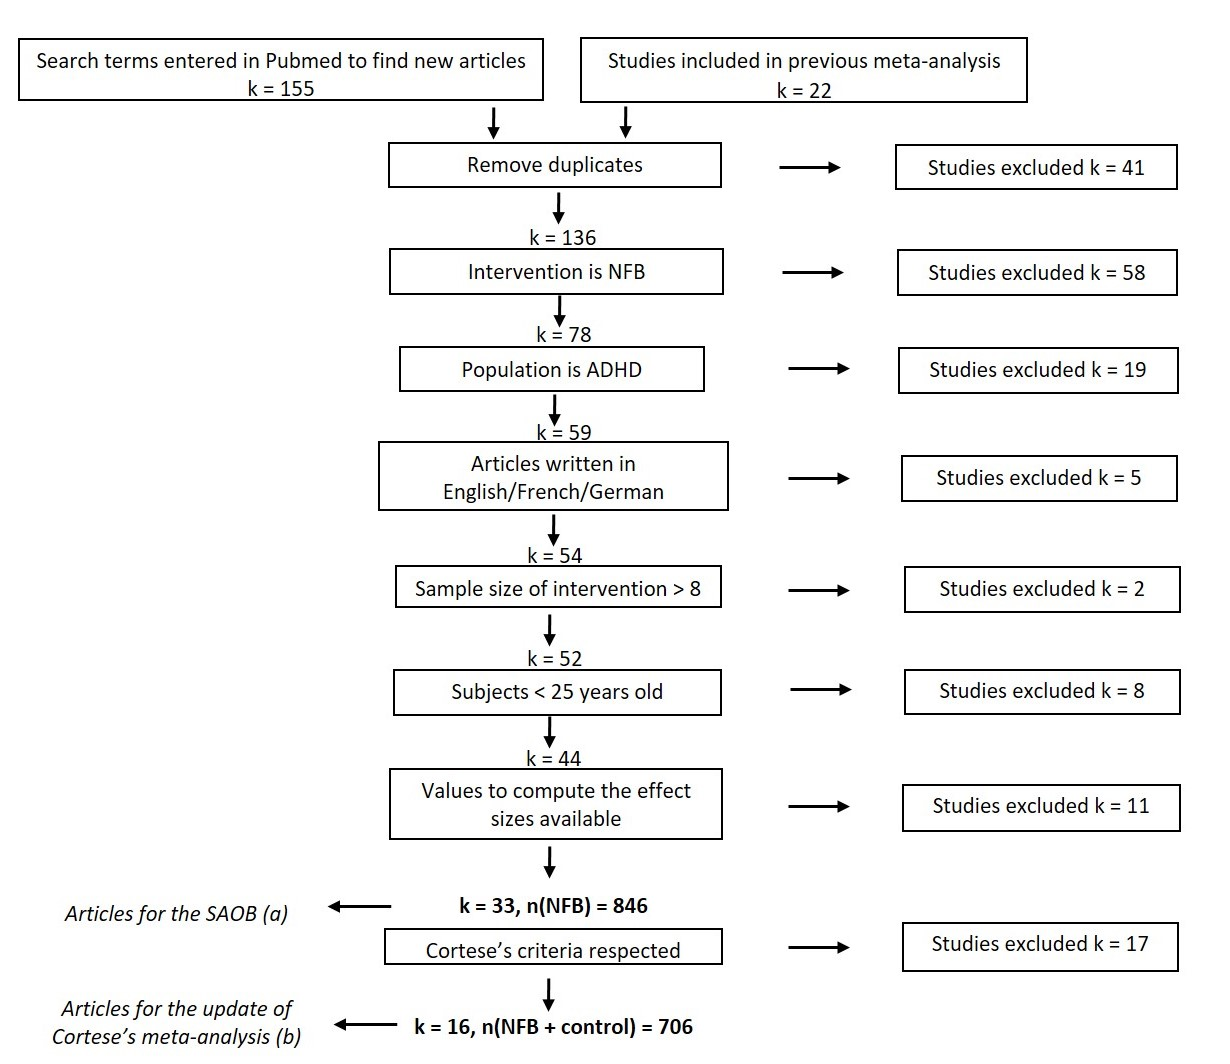
\includegraphics[width=1.0\linewidth]{figures/meta_review_factors_analysis_how_studies_are_included_no_colors_2-columns_fitting_ima.jpg} 
  \caption{Flow diagram of selection of studies (last search on February 12, 2018).  
	The subset (a) corresponds to the \citeauthor{Cortese2016}'s inclusion criteria without the requirement for 
	the presence of a control group.
	The subset (b) exactly corresponds to the studies included in \citet{Cortese2016} and more recent work meeting the same criteria.}
  \label{Figure:systematic_review_workflow}
\end{figure}

\begin{figure}[h!]
  \centering
  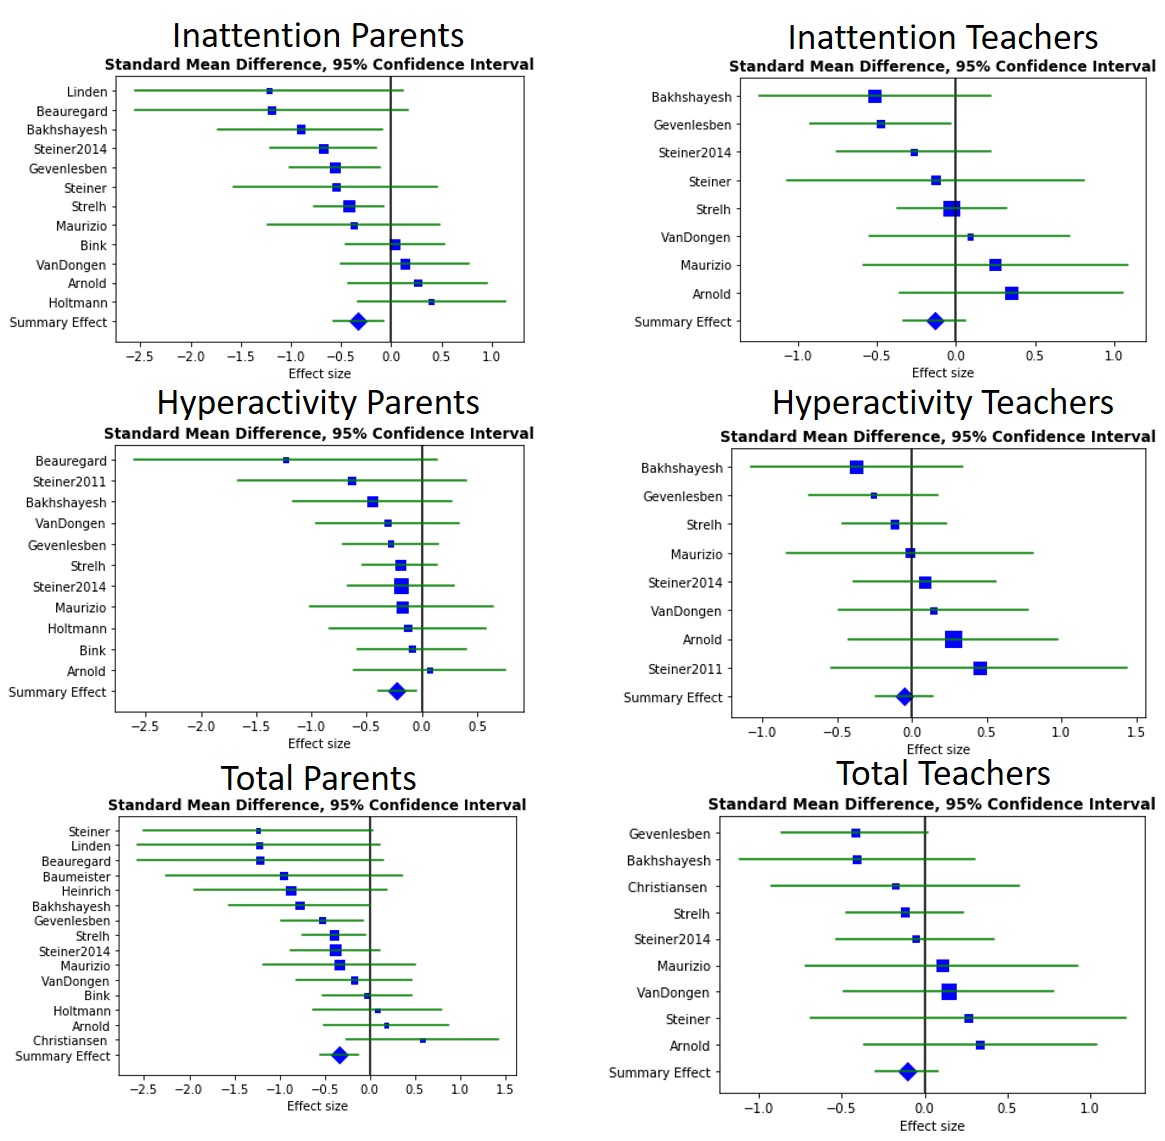
\includegraphics[width=1.0\linewidth]{figures/meta_review_forest_plots_update_meta_analysis_our_choices_no_colors_2-columns_fitting_image.jpg}
  \caption{Forest plots showing the between-\glsfirst{es}. A negative \gls{es} is in favor of \glsfirst{nfb}. 
	The blue squares correspond of the \gls{es}, the blue diamond to the \glsfirst{se} and the green line to the 95\% confidence interval.}
  \label{Figure:meta_review_forest_plots_update_meta_analysis_our_choices_no_colors_2-columns_fitting_image}
\end{figure}

\begin{figure}[h!]
  \centering
  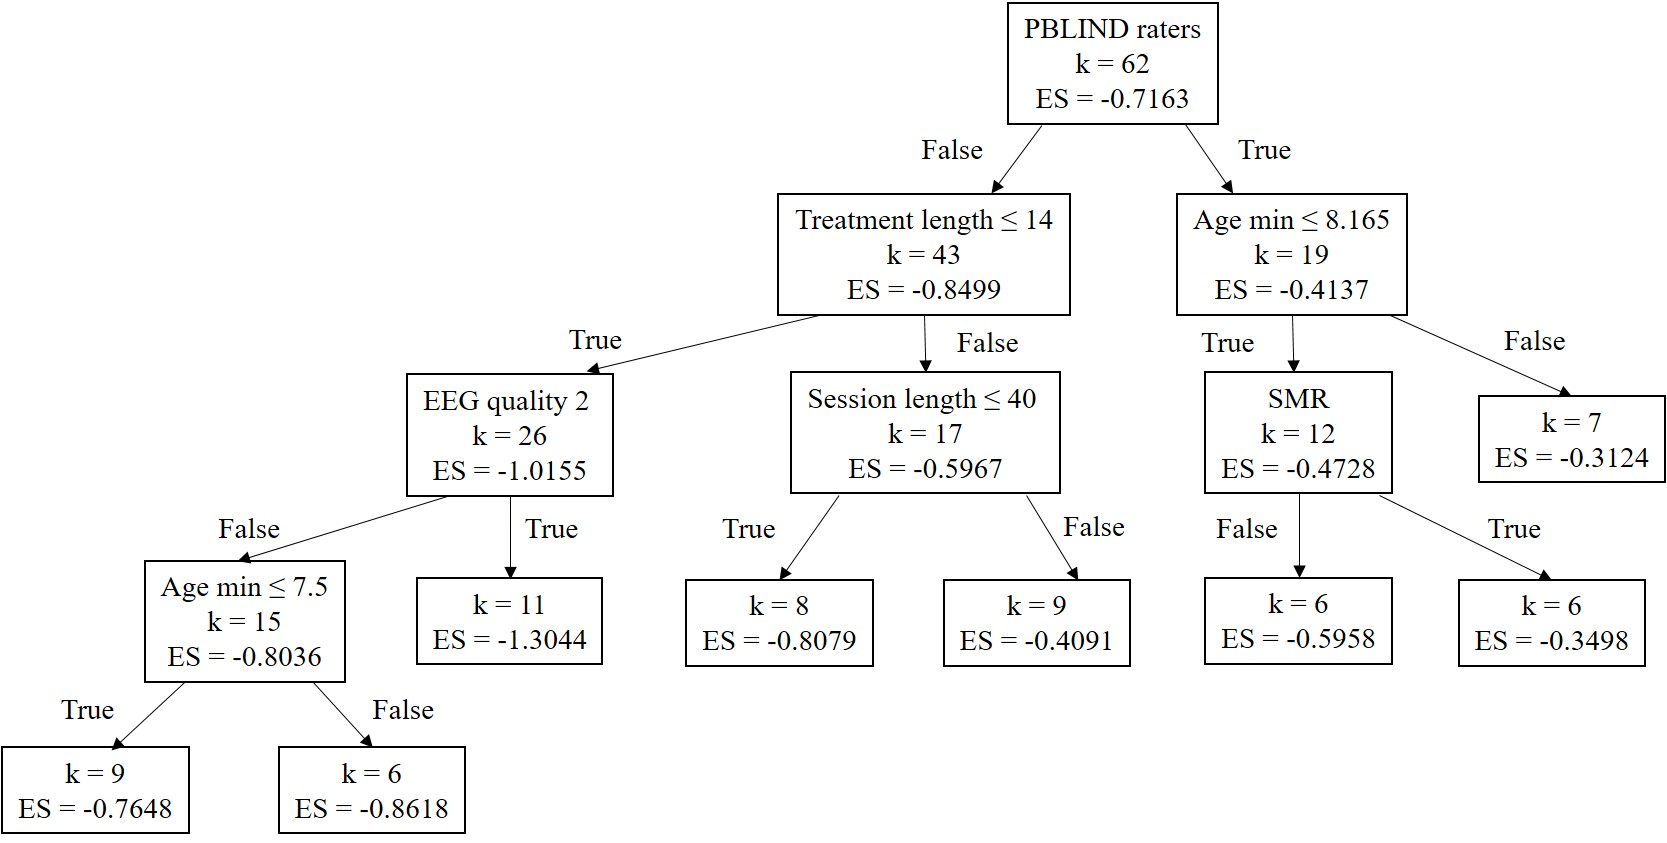
\includegraphics[width=1.0\linewidth]{figures/factors_analysis_decision_tree_results_no_colors_2-columns_fitting_image.jpg}
  \caption{Decision Tree obtained: \glsfirst{es} corresponds to the within subject effect size and $k$ to the number of studies, 
  The importance of variables is decreasing from top to bottom.
	from the root node.}
  \label{Figure:factors_analysis_decision_tree_results}
\end{figure}

\begin{figure}[h!]
  \centering
  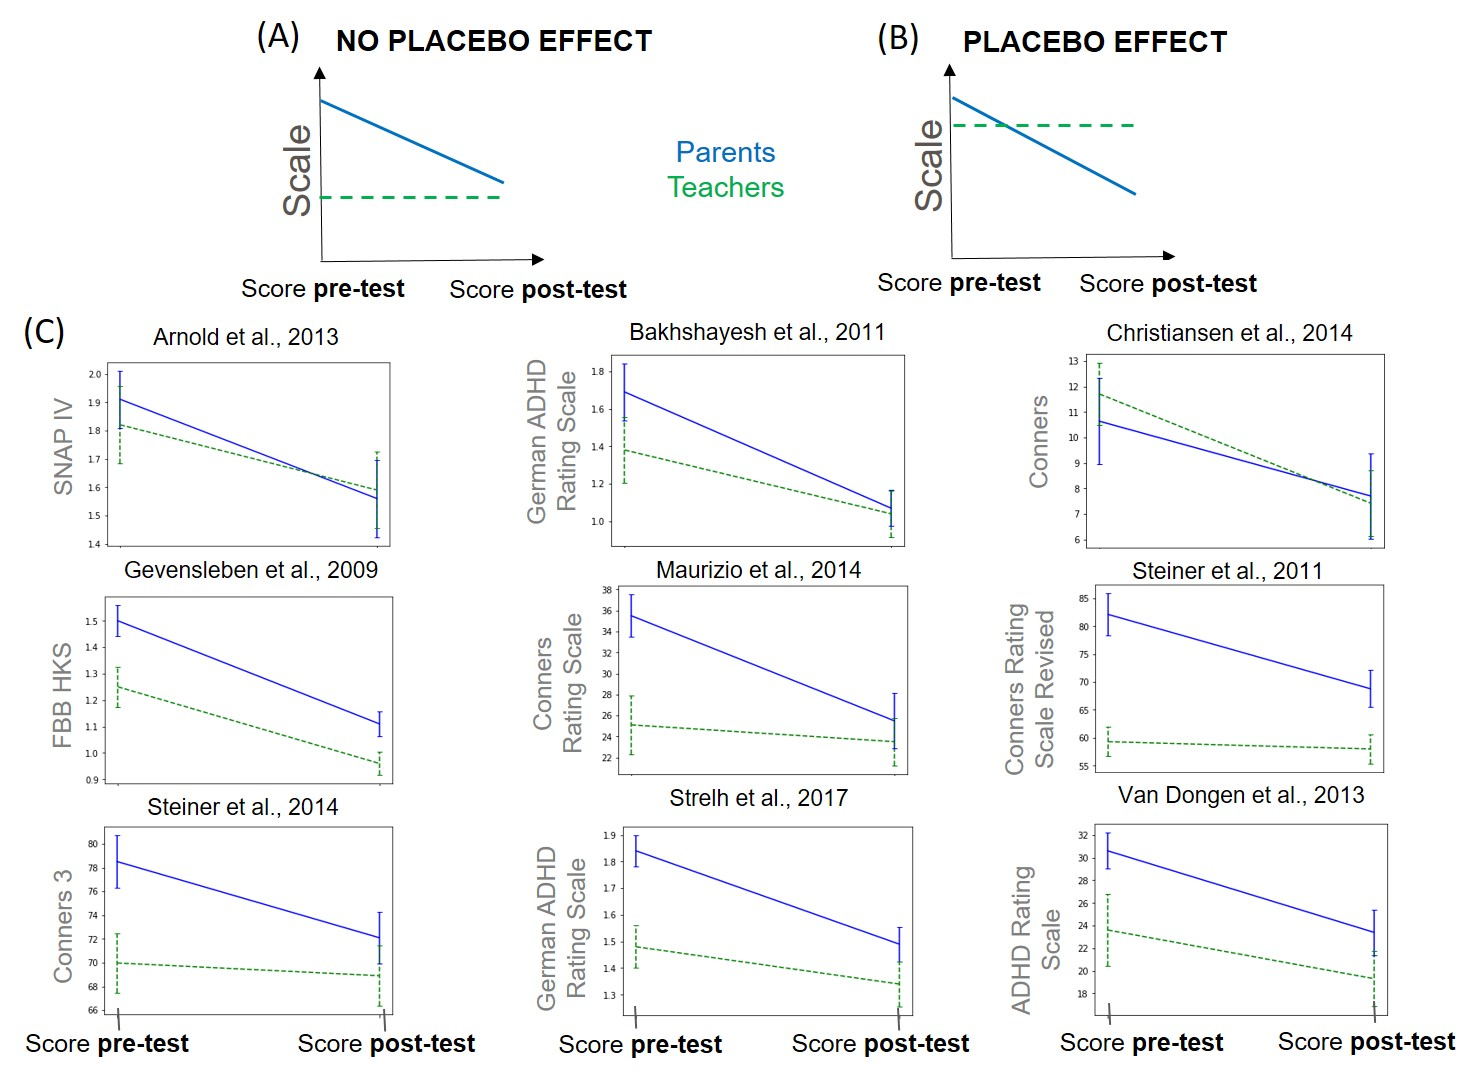
\includegraphics[width=1.0\linewidth]{figures/discussion_on_placebo_effect_colors_2-columns_fitting_image.jpg}
  \caption{Pre-test and post-test scores ($\pm$ standard error) given by Parents (\glsfirst{mprox}) in blue and teachers (\glsfirst{pblind}) in green, dashed line. 
	Data hypothesized under 2 different hypothesis: \textbf{(A)} teachers see less symptoms altogether so that difference pre-post is low and \textbf{(B)}
	Placebo: teacher see as much baseline symptoms as parents but don't see as much improvement as they do. \textbf{(C)} Real data: evolution of parents 
	and teachers' scores between pre and post-test on studies that satisfy \citeauthor{Cortese2016}'s inclusion criteria and that provide teachers and parents
	scores on the same scale.}
  \label{Figure:discussion_on_placebo_effect_colors_2-columns_fitting_image}
\end{figure} 
